% begin module integral-test-above
\begin{frame}
\begin{columns}
\column{.6\textwidth}
\[
\sum_{n=1}^\infty \frac{1}{n^2} = \alert<handout:0| 6-10,14>{\frac{1}{1^2}} \alert<handout:0| 7-10,14>{+\alert<handout:0| 13>{\frac{1}{2^2}}} \alert<handout:0| 8-10,13-14>{+ \frac{1}{3^2}} \alert<handout:0| 9-10,13-14>{+ \frac{1}{4^2}} \alert<handout:0| 10,13-14>{+ \cdots} 
\]
\begin{itemize}
\item<2->  Use a computer to calculate partial sums.
\item<3->  Looks like it's converging.
\item<4->  How do we prove it?
\item<5->  Use $f(x) = \frac{1}{x^2}$.
\end{itemize}
\begin{center}
\uncover<5->{%
\only<handout:0| -5>{%
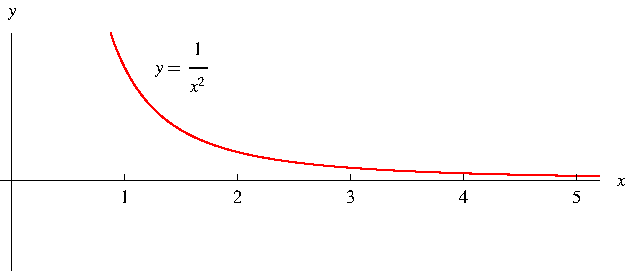
\includegraphics[width=6.5cm]{series/pictures/12-03-integral-test-abovea.pdf}%
}%
}%
\only<handout:0| 6>{%
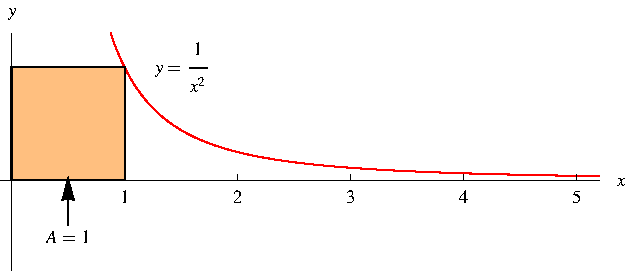
\includegraphics[width=6.5cm]{series/pictures/12-03-integral-test-aboveb.pdf}%
}%
\only<handout:0| 7>{%
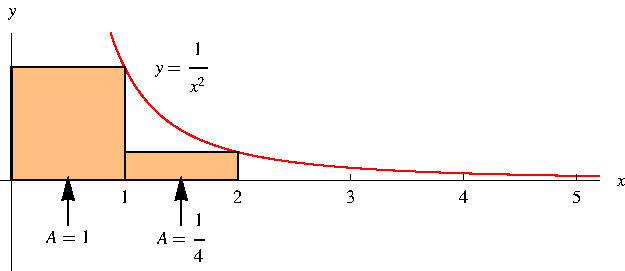
\includegraphics[width=6.5cm]{series/pictures/12-03-integral-test-abovec.pdf}%
}%
\only<handout:0| 8>{%
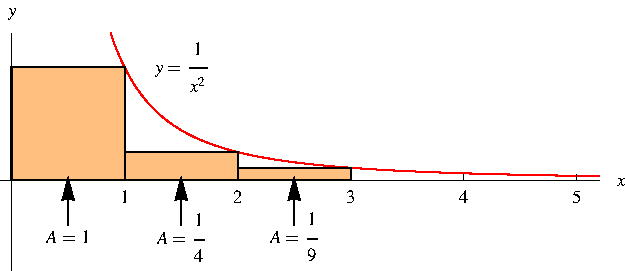
\includegraphics[width=6.5cm]{series/pictures/12-03-integral-test-aboved.pdf}%
}%
\only<handout:0| 9>{%
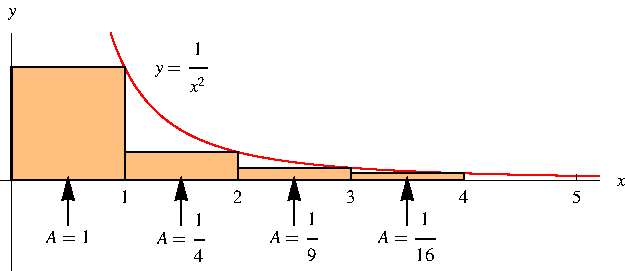
\includegraphics[width=6.5cm]{series/pictures/12-03-integral-test-abovee.pdf}%
}%
\only<handout:1| 10-11>{%
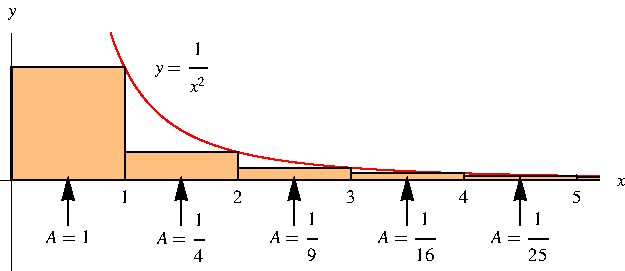
\includegraphics[width=6.5cm]{series/pictures/12-03-integral-test-aboveg.pdf}%
}%
\only<handout:2| 12>{%
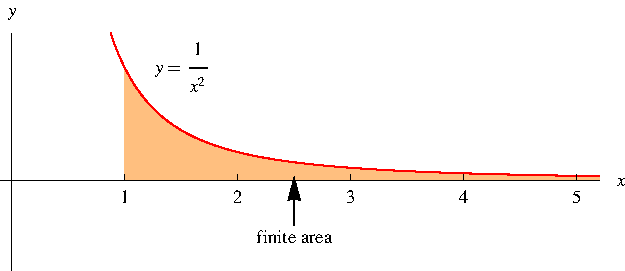
\includegraphics[width=6.5cm]{series/pictures/12-03-integral-test-aboveh.pdf}%
}%
\only<handout:3| 13>{%
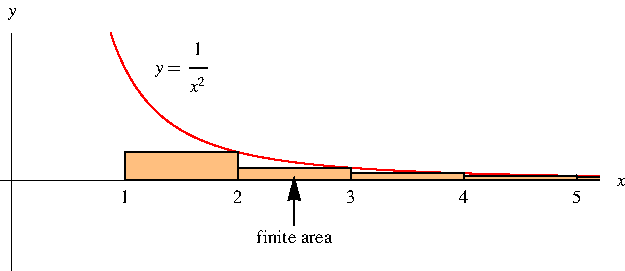
\includegraphics[width=6.5cm]{series/pictures/12-03-integral-test-abovei.pdf}%
}%
\only<handout:4| 14>{%
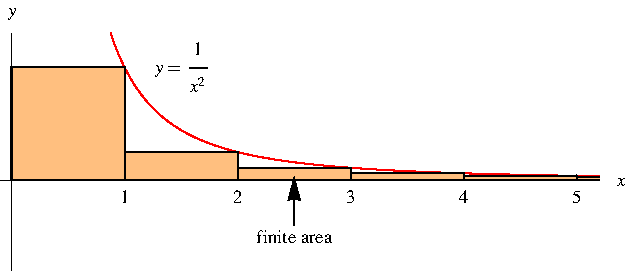
\includegraphics[width=6.5cm]{series/pictures/12-03-integral-test-abovej.pdf}%
}%
\end{center}
\column{.4\textwidth}
\uncover<2->{%
\[
\begin{array}{|r@{\ }|c|}
\hline
n & s_n = \sum_{i=1}^n \frac{1}{i^2}\\
\hline
     5 & 1.4636 \\
    10 & 1.5498 \\
    50 & 1.6251 \\
   100 & 1.6350 \\
   500 & 1.6429 \\
  1000 & 1.6439 \\
  5000 & 1.6447 \\
\hline
\end{array}
\]
}%
\begin{itemize}
\item<6->  $\frac{1}{1^2}$ is the area of a rectangle.
\item<7->  So is $\frac{1}{2^2} = \frac{1}{4}$.
\item<handout:2-| 11-| alert@11-12>  The improper integral $\int_1^\infty \frac{1}{x^2}\diff x$ is \uncover<12->{convergent.}
\item<handout:4-| 14->  Therefore $\sum_{n=1}^\infty \frac{1}{n^2}$ is convergent.
\end{itemize}
\end{columns}
\end{frame}
% end module integral-test-above
